\begin{figure}[!h]
\centering
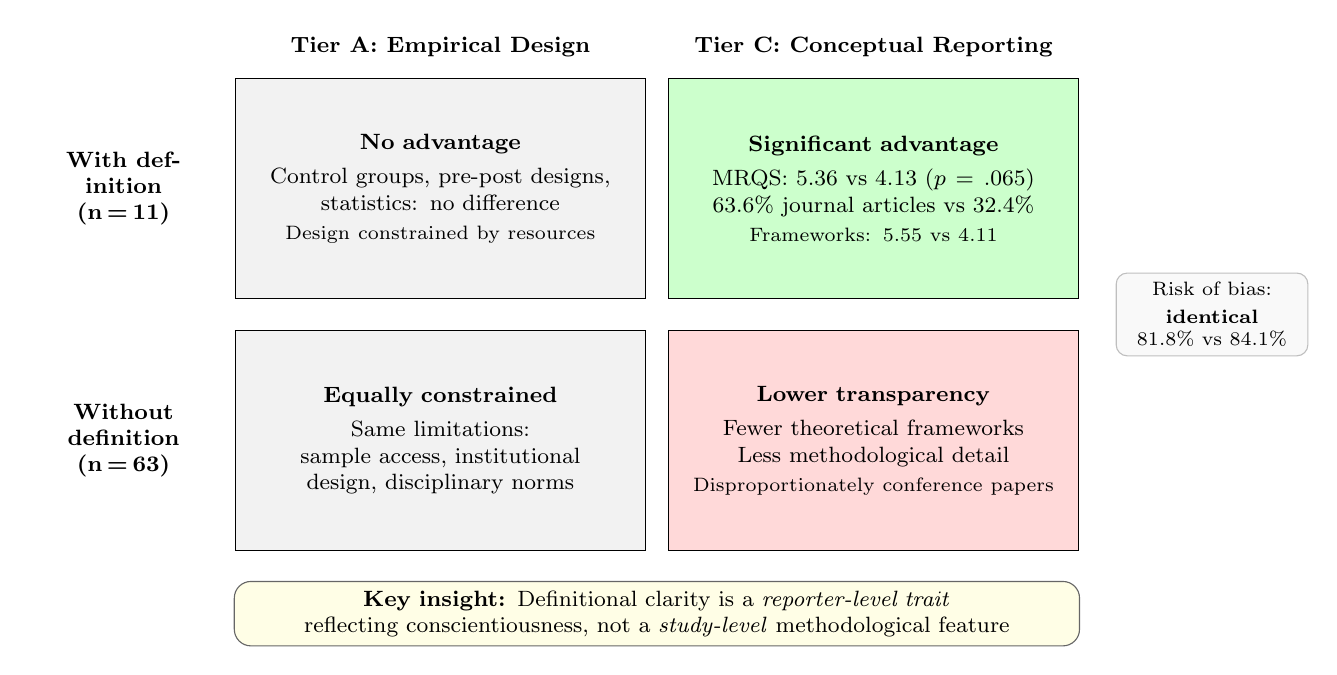
\begin{tikzpicture}[
  cell/.style={
    draw, minimum width=5.2cm, minimum height=2.8cm,
    text width=4.7cm, align=center, font=\footnotesize
  },
  header/.style={
    font=\footnotesize\bfseries, align=center
  },
]

% Column headers
\node[header] at (2.6, 1.8) {Tier~A: Empirical Design};
\node[header] at (8.1, 1.8) {Tier~C: Conceptual Reporting};

% Row headers — anchored east, clear of cells
\node[header, text width=2.2cm, anchor=east] at (-0.2, 0) {With definition\\(n\,=\,11)};
\node[header, text width=2.2cm, anchor=east] at (-0.2, -3.2) {Without definition\\(n\,=\,63)};

% Top-left: With definition × Tier A
\node[cell, fill=gray!10] (tl) at (2.6, 0) {%
  \textbf{No advantage}\\[3pt]
  Control groups, pre-post designs,\\
  statistics: no difference\\[1pt]
  {\scriptsize Design constrained by resources}%
};

% Top-right: With definition × Tier C
\node[cell, fill=green!20] (tr) at (8.1, 0) {%
  \textbf{Significant advantage}\\[3pt]
  MRQS: 5.36 vs 4.13 ($p = .065$)\\
  63.6\% journal articles vs 32.4\%\\[1pt]
  {\scriptsize Frameworks: 5.55 vs 4.11}%
};

% Bottom-left: Without definition × Tier A
\node[cell, fill=gray!10] (bl) at (2.6, -3.2) {%
  \textbf{Equally constrained}\\[3pt]
  Same limitations:\\
  sample access, institutional\\
  design, disciplinary norms%
};

% Bottom-right: Without definition × Tier C
\node[cell, fill=red!15] (br) at (8.1, -3.2) {%
  \textbf{Lower transparency}\\[3pt]
  Fewer theoretical frameworks\\
  Less methodological detail\\[1pt]
  {\scriptsize Disproportionately conference papers}%
};

% Right annotation: RoB
\node[
  draw=gray!50, rounded corners=4pt, fill=gray!5,
  text width=2.2cm, align=center, font=\scriptsize
] at (12.4, -1.6) {%
  Risk of bias:\\[2pt]
  \textbf{identical}\\
  81.8\% vs 84.1\%%
};

% Bottom insight box
\node[
  draw=black!60, rounded corners=6pt, fill=yellow!10,
  text width=10.5cm, align=center, font=\footnotesize
] at (5.35, -5.4) {%
  \textbf{Key insight:} Definitional clarity is a \emph{reporter-level trait}\\
  reflecting conscientiousness, not a \emph{study-level} methodological feature%
};

\end{tikzpicture}
\caption{Interaction between definitional practices and quality dimensions. Studies with explicit definitions score higher on conceptual reporting items (Tier~C, right column) but show no advantage on empirical design items (Tier~A, left column). Risk of bias is effectively identical regardless of definitional practices. This pattern reveals that definitional clarity operates as a reporter-level trait reflecting conscientiousness, not as a driver of stronger study design (see Section~\ref{sec:def-quality}).}
\label{fig:definitional-quality-interaction}
\end{figure}
